
\section{Neural module networks for visual QA}
\label{sec:model}

%Given a pre-trained \emph{network layout predictor} $P$, 
Each training datum for this task can be thought of as a 3-tuple $(w, x, y)$, where
\begin{itemize}
  \setlength\itemsep{0em}
  \item $w$ is a natural-language question
  %\item $p = P(w)$ a network layout
  \item $x$ is an image
  \item $y$ is an answer
\end{itemize}
A model is fully specified by a collection of modules $\{ m \}$, each with
associated parameters $\theta_m$, and a \emph{network layout predictor} $P$
which maps from strings to networks.. Given $(w, x)$ as above, the model
instantiates a network based on $P(w)$, passes $x$ (and possibly $w$ again) as
inputs, and obtains a distribution over labels (for the VQA task, we require the
output module to be a classifier). Thus a model ultimately encodes a predictive
distribution $p(y\ |\ w,\ x;\ \theta)$.

In the remainder of this section, we describe the set of modules used for the
VQA task, then explain the process by which questions are converted to network
layouts.

\subsection{Modules}

Our goal here is to identify a small set of modules that can be assembled into
all the configurations necessary for our tasks. This corresponds to identifying
a minimal set of composable vision primitives. The modules operate on three
basic data types: images, unnormalized attentions, and labels.  For the
particular task and modules described in this paper, almost all interesting
compositional phenomena occur in the space of attentions, and it is not
unreasonable to characterize our contribution more narrowly as an
``attention-composition'' network. Nevertheless, other types may be required in
the future (for different new or for greater coverage in the VQA domain).

First, some notation: module names are typeset in a {\tt fixed width font}, and
are of the form \mod{TYPE[INSTANCE](ARG$_1$, \ldots)}. \mod{TYPE} is a
high-level module type (attention, classification, etc.) of the kind described
in this section. \mod{INSTANCE} is the particular instance of the model under
consideration---for example, \mod{attend[red]} locates red things, while
\mod{attend[dog]} locates dogs. Weights may be shared at both the type and
instance level. Modules with no arguments implicitly take the image as input;
higher-level arguments may also inspect the image.

\pagebreak
\subsubsection*{Attention}
\[
  \mod{attend} : \mathit{Image} \to \mathit{Attention}
\]
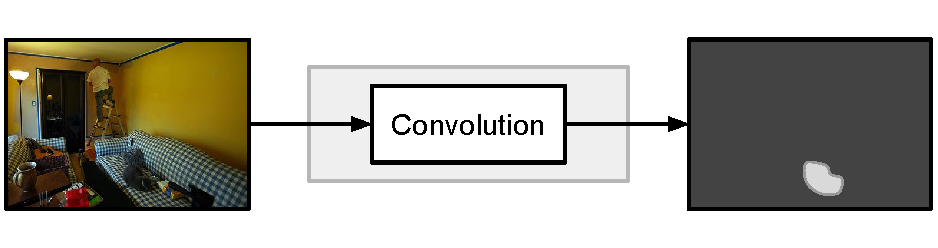
\includegraphics[width=\columnwidth]{fig/attend}
An attention module \mod{attend[$c$]} convolves every position in the input
image with a weight vector (distinct for each $c$) to produce a heatmap or
unnormalized attention. So, for example, the output of the module {\small\tt
attend[dog]} is a matrix whose entries should be in regions of the image
containing cats, and small everywhere else, as shown above.\\

\subsubsection*{Re-attention}
\[
  \mod{re-attend} : \mathit{Attention} \to \mathit{Attention}
\]
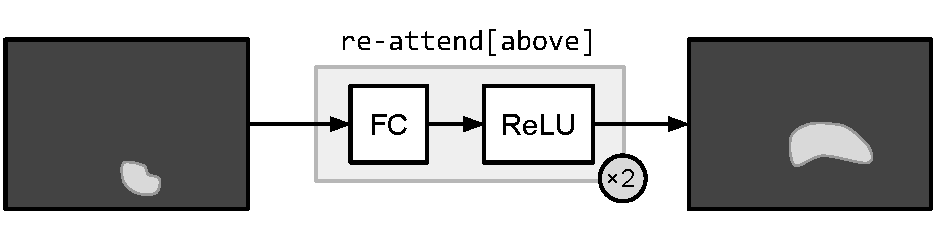
\includegraphics[width=\columnwidth]{fig/re-attend}
A re-attention module \mod{re-attend[$c$]} is essentially just a multilayer
perceptron, performing a fully-connected mapping from one attention to another.
Again, the weights for this mapping are distinct for each $c$. So
\mod{re-attend[above]} should take an attention and shift the regions of
greatest activation upward (as above), while \mod{re-attend[not]} should move
attention away from the active regions. For the experiments in this paper, the
first FC layer produces a vector of size 32, and the second is the same size as
the input. \\%[1em]

\subsubsection*{Combination}
\[
  \mod{combine} : \mathit{Attention} \times \mathit{Attention} \to
  \mathit{Attention}
\]
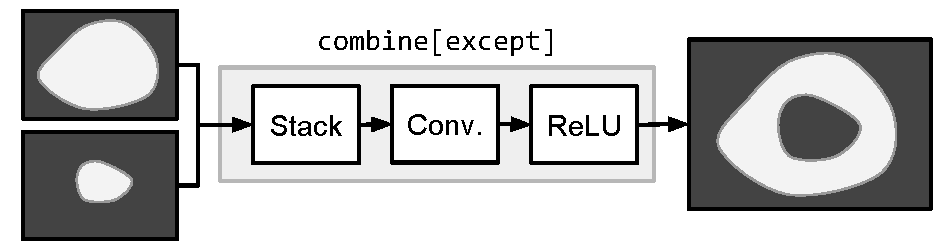
\includegraphics[width=\columnwidth]{fig/combine}
A combination module \mod{combine[$c$]} merges two attentions into a single
attention. For example, {\small\tt combine[and]} should be active only in the
regions that are active in both inputs, while {\small\tt{combine[except]}}
should be active where the first input is active and the second is
inactive.

\subsubsection*{Classification}
\[
  \mod{classify} : \mathit{Image} \times \mathit{Attention} \to
  \mathit{Label}
\]
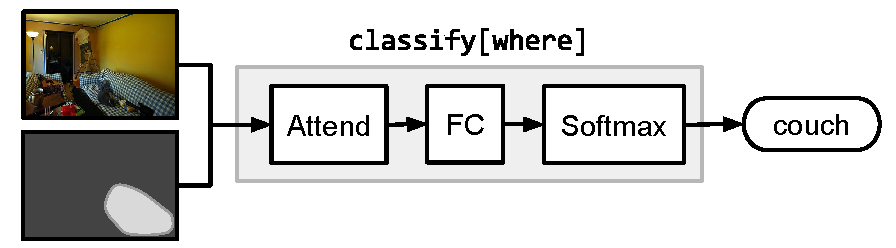
\includegraphics[width=\columnwidth]{fig/classify}
A classification module \mod{classify[$c$]} takes an attention and the input
image and maps them to a distribution over labels. For example, {\small\tt
classify[color]} should return a distribution over colors for the region
attended to.

\subsubsection*{Measurement}
\[
  \mod{measure} : \mathit{Attention} \to \mathit{Label}
\]
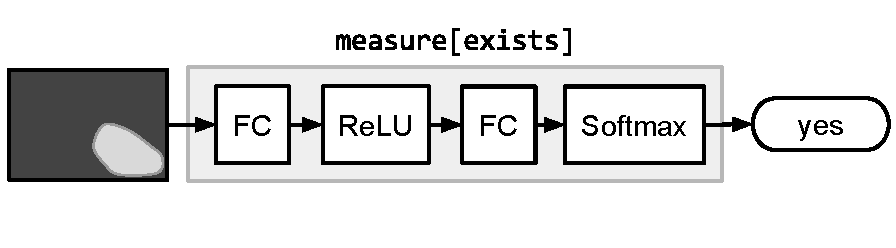
\includegraphics[width=\columnwidth]{fig/measure}
A measurement module \mod{measure[$c$]} takes an attention alone and maps it to
a distribution over labels. Because attentions passed between modules are
unnormalized, \mod{measure} is suitable for evaluating the existence of a
detected object, or counting sets of objects.

\begin{figure*}
  \begin{subfigure}[t]{0.4\textwidth}
    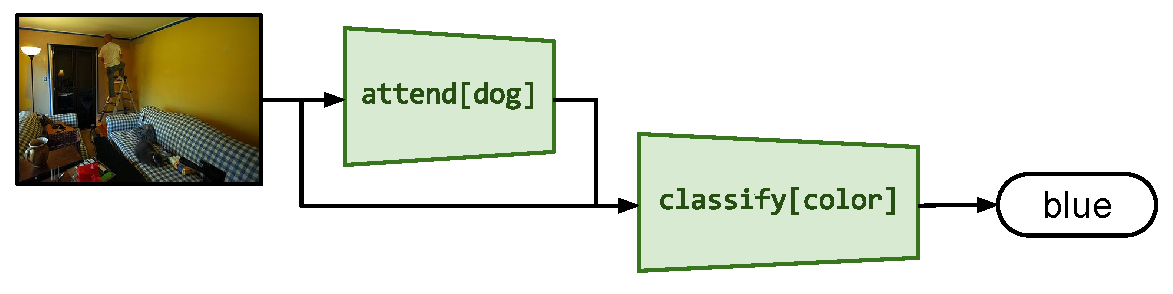
\includegraphics[width=\textwidth]{fig/full1}
    \caption{NMN for answering the question \emph{What color is
    his tie?} The \mod{attend[tie]} module first predicts a heatmap
    corresponding to the location of the tie. Next, the \mod{classify[color]}
    module uses this heatmap to produce a weighted average of image features,
  which are finally used to predict an output label.}
  \end{subfigure}
  \hfill
  \begin{subfigure}[t]{0.55\textwidth}
    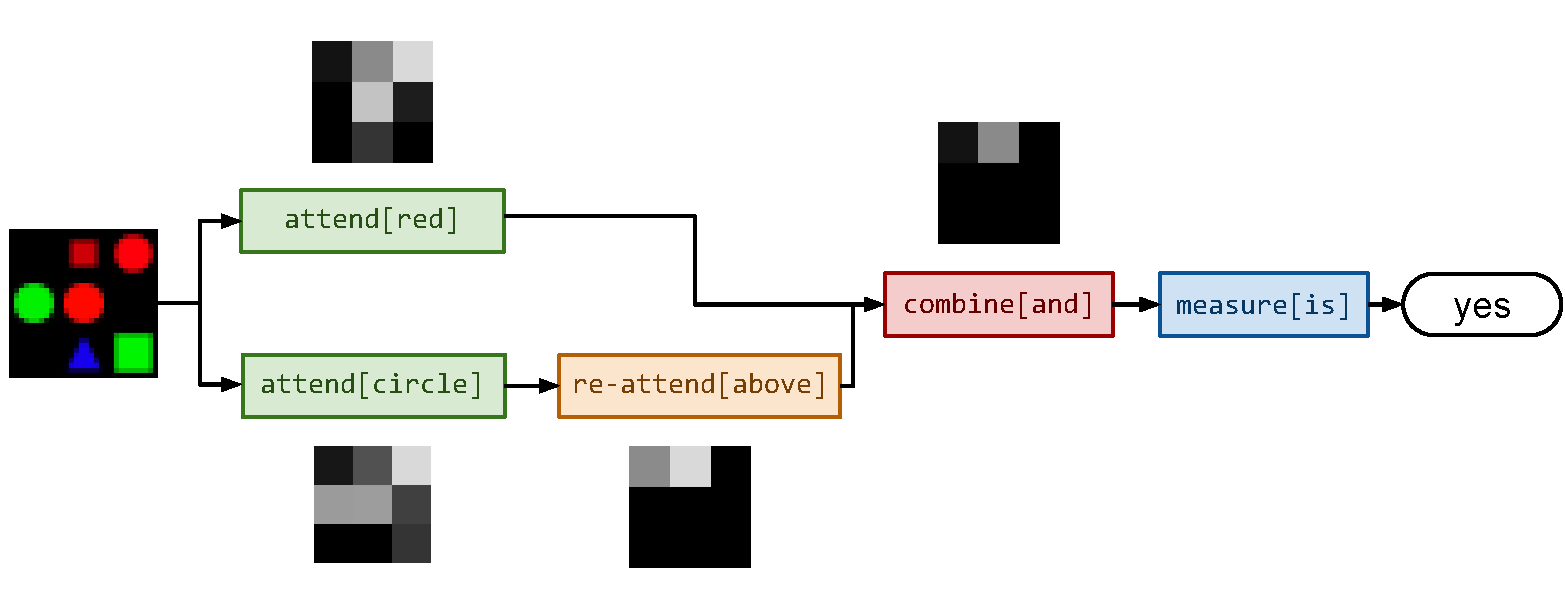
\includegraphics[width=\textwidth]{fig/full2}
    \caption{NMN for answering the question \emph{Is there a red shape above a
    circle?} The two \mod{attend} modules locate the red shapes and circles,
    the \mod{re-attend[above]} shifts the attention above the circles, the
    \emph{combine} module computes their intersection, and the
    \mod{measure[is]} module inspects the final attention and determines
  that it is non-empty.}
  \label{fig:shape-nmn}
  \end{subfigure}
  \caption{Sample NMNs for question answering about natural images and shapes.
  For both examples, layouts attentions and answers are real predictions made by
  our model.}
  \label{fig:nmns}
\end{figure*}


\subsection{From strings to networks}

The transformation from a natural language question to an instantiated neural
network takes place in two steps.  First we map from natural language questions
to \emph{layouts}, which specify both the set of modules used to answer a given
question, and the connections between them. Next we use these layouts are used
to assemble the final prediction networks.

We use standard tools pre-trained on existing linguistic resources to obtained
structured representations of questions. Future work might focus on learning (or
at least fine-tuning) this prediction process jointly with the rest of the
system. %, though in fact off-the-shelf tools produce high-quality analyses for
%almost all the questions in our data.

\paragraph{Parsing}
Specifically, we begin by parsing each question with the Stanford Parser
\cite{Klein03Unlex}.
to obtain a universal dependency representation \cite{DeMarneffe08Deps}.
Dependency parses express grammatical relations between parts of a sentence
(e.g.\ between objects and their attributes, or events and their participants),
and provide a lightweight abstraction away from the surface form of the
sentence. The parser also performs basic lemmatization, for example turning
\emph{kites} into \emph{kite} and \emph{were} into \emph{be}. 

Next, we filter the set of dependencies to those connected the wh-word in the
question (the exact distance we traverse varies depending on the task). This
gives a simple logical form expressing (the primary) part of the sentence's
meaning.  For example, \emph{what is standing in the field} becomes
\mod{what(stand)}; \emph{what color is the truck} becomes \mod{color(truck)},
and \emph{is there a circle next to a square} becomes \mod{is(cicle,
next-to(square))}.
In the process we also strip away function words like determiners and
modals, so \emph{what type of cakes were they?} and \emph{what type of cake is
it?} both get converted to \mod{type(cake)}.

It is easiest to think of these representations as pieces of a variable-free
combinatory logic \cite{Liang13DCS}; every leaf is implicitly a function taking
the image as input. The code for transforming parse trees to structured queries
will be provided in the accompanying software package.

\paragraph{Layout}
These logical forms already determine the structure of the predicted network,
but not the identities of the modules that compose it. This final assignment of
modules is fully determined by the structure of the parse. All leaves become
\mod{attend} modules, all internal nodes become \mod{re-attend} or \mod{combine}
modules dependint on their arity, and root nodes become \mod{measure} modules
for yes/no questions and \mod{classify} modules for all other quesiton types.

Given the mapping from queries to network layouts described above, we have for
each training example a network structure, an input image, and an output label.
In many cases, these network structures are different, but have tied parameters.
Networks which have the same high-level structure but different instantiations
of individual modules (for example \emph{what color is the cat?}---{\small\tt
classify[color](attend[cat])} and \emph{where is the truck?}---{\small\tt
classify[where](attend[truck])}) can be processed in the same batch, resulting
in efficient computation.

As noted above, parts of this conversion process are task-specific---we found
that relatively simple expressions were best for the natural image questions,
while the shapes question (by design) required deeper structures. Some summary
statistics are provided in \autoref{tab:struct-summary}.

\begin{table*}
  \centering
  \begin{tabular}{cccccc}
    \toprule
    & \# types & \# instances & \# layouts & max depth & max size \\
    \midrule
    VQA & 4 & 1995 & 66549 & 2 & 3 \\
    \cocoqa & 3 & 892 & 4613 & 2 & 2\\
    \shapes & 4 & 8 & 164 & 5 & 6 \\
    \bottomrule
  \end{tabular}
  \caption{Structure summary statistics for neural module networks used in this
    paper. ``\# types'' is the number of high-level module types available (e.g.
    \emph{attend}), ``\# instances'' is the number of specific module instances
    (e.g. \mod{attend[llama]}), and ``\# layouts'' is the number of distinct
    composed structures (e.g. \mod{classify[color](attend[llama])}).
    ``Max depth'' is the greatest depth across all layouts, while ``max
    size'' is the greatest number of modules---for example, the network in
    \autoref{fig:shape-nmn}
    has depth 4 and size 5. (All numbers from training sets.)
  }
  \label{tab:struct-summary}
\end{table*}


\paragraph{Generalizations}

It is easy to imagine applications where the input to the layout stage comes
from something other than a natural language parser. Users of an image database,
for example, might write SQL-like queries directly in order to specify their
requirements precisely, e.g.
\begin{flushleft}
  {\tt IS(cat) AND NOT(IS(dog))}
\end{flushleft}
or even mix visual and non-visual specifications in their queries:
\begin{flushleft}
  {\tt IS(cat) and date > 2014-11-5}
\end{flushleft}

Indeed, it is possible to construct this kind of ``visual SQL'' using precisely
the approach described in this paper---once our system is trained, the learned
modules for attention, classification, etc. can be assembled by any kind of
outside user, without relying on natural language specifically.

\subsection{Integrating common-sense knowledge}

So far our discussion has focused on the neural module net architecture, without
reference to the remainder of \autoref{fig:teaser}. Our final model combines the output
from the neural module network with predictions from a simple LSTM question
encoder. This is important for two reasons. First, because of the relatively
aggressive simplification of the question that takes place in the parser,
grammatical cues that don't substantively change the semantics of the question,
but which might affect the answer, are discarded. For example, \emph{what is
flying?} and \emph{what are flying?} both get converted to \mod{what(fly)}, but
their answers should be \emph{kite} and \emph{kites} respectively, even given
the same underlying image features. The question encoder thus allows us to model
underlying syntactic regularities in the data. Second, it allows us to capture
\emph{semantic} regularities: with missing or low-quality image data, it is
reasonable to guess that \emph{what color is the bear?} is answered by
\emph{brown}, and unreasonable to guess \emph{green}. The question encoder also
allows us to model effects of this kind.

All experiments in this paper use a standard single-layer LSTM with 1024 hidden
units.

\section{Training neural module networks}

Our training objective is simply to find module parameters maximizing the
likelihood of the data. By design, the last module in every network is a
{\small\tt classify}, and so each assembled network represents a probability
distribution.

Because of the dynamic network structures used to answer questions, some weights
are updated much more frequently than others. For this reason we found that
learning algorithms with adaptive per-weight learning rates performed
substantially better than simple gradient descent. All the experiments described
below use AdaDelta \cite{Zeiler12Adadelta}  (thus there was no hyperparameter
search over step sizes).

It is important to emphasize that the labels we have assigned to distinguish
instances of the same module type---\mod{cat}, \mod{and}, etc.---are a
notational convenience, and do not reflect any manual specification of the
behavior of the corresponding modules. \mod{detect[cat]} is not fixed or even
initialized %doesn't know it's
as cat recognizer (rather than a couch recognizer or a dog recognizer), and
\mod{combine[and]} isn't fixed to compute intersections of attentions (rather
than unions or differences). Instead, they acquire these behaviors as a
byproduct of the end-to-end training procedure. As can be seen in
\autoref{fig:nmns},
the image--answer pairs and parameter tying together encourage each module to
specialize in the appropriate way.
